\documentclass[11pt,a4paper]{article}
\usepackage[margin=1in]{geometry}
\usepackage{amsmath,amssymb}
\usepackage{graphicx}
\usepackage{float}
\usepackage{enumitem}
\usepackage{microtype}
\usepackage{caption}
\usepackage{tabularx}
\usepackage{hyperref}

\captionsetup{font=small,labelfont=bf,skip=6pt}

\setlist[itemize]{leftmargin=1.2cm}
\setlist[enumerate]{leftmargin=1.2cm}

\newcommand{\problembox}[3]{%
  \par\addvspace{0.42em}%
  \noindent
  \setlength{\fboxsep}{7.5pt}%
  \setlength{\fboxrule}{0.95pt}%
  \fbox{%
    \begin{minipage}{\dimexpr\linewidth-2\fboxsep-2\fboxrule\relax}
    \begin{tabularx}{\linewidth}{@{}>{\raggedright\arraybackslash\bfseries}p{2.1em} @{\hspace{0.9em}} >{\raggedright\arraybackslash}X @{\hspace{0.9em}} >{\raggedleft\arraybackslash\bfseries}p{2.4em}@{}}
    #1 & #2 & #3
    \end{tabularx}
    \end{minipage}%
  }%
  \par\addvspace{0.32em}%
}

\title{\textbf{Fluorescence}}
\author{\normalsize Y25 (2025) --- English translation}
\date{}
\begin{document}
\maketitle

\section*{Equipment}

\textbf{Electrical:} Photosensitive CCD ruler connected to a computer, magnetic screen, USB flash drive, USB lamp.

\begin{figure}[H]
    \centering
    
\includegraphics[width=0.72\textwidth]{E3_EN_assets/fig1.jpg}
    \caption{Electrical equipment.}
\end{figure}

\textbf{Optical:} Power supply (15 V), cable adapter, continuous spectrum LED (LED-CON), three-color LED (LED-RGB), three black lenses $L_1$ (+6 D), one white lens $L_2$ (+16 D), lens $L_3$ on a rod, diffraction grating ($d_0=2.0$ $\mu$m), optical table, stand for illuminator and cuvettes, spacer, stand for lens $L_3$ and laser, ruler, slit.

\begin{figure}[H]
    \centering
    
\includegraphics[width=0.72\textwidth]{E3_EN_assets/fig2.jpg}
    \caption{Optical equipment.}
\end{figure}

\textbf{Chemical:} 10 cuvettes with lids, analysis jars with water, 0.5 ml syringe, two 3 ml syringes, red/green/blue lasers, batteries, laser button holder, Rhodamine B solution ($c_0=200$ $\mu$M), tweezers.

\begin{figure}[H]
    \centering
    
\includegraphics[width=0.72\textwidth]{E3_EN_assets/fig3.jpg}
    \caption{Chemical equipment.}
\end{figure}

\section*{Introduction}

The Jablonski diagram is used to represent energy states. For Rhodamine B (RhB), the total energy $E$ is the sum of electronic energy $E_e$ and atomic vibration energy $E_a$ ($E_a \ll E_e$). $S_0$ is the ground state (energies set to zero). $S_1$ is the first excited electronic state. Vibrational levels are denoted by $\nu$.

\begin{figure}[H]
    \centering
    
\includegraphics[width=0.72\textwidth]{E3_EN_assets/fig4.jpg}
    \caption{Jablonski diagram levels.}
\end{figure}

The photon energy is $\hbar \omega$. If a molecule is in $S_0, \nu=0$, it can absorb a photon if $\hbar \omega = E_1 - E_2$. Absorption and emission lines are broadened; the width is characterized by the FWHM (Full Width at Half Maximum).

\begin{figure}[H]
    \centering
    
\includegraphics[width=0.72\textwidth]{E3_EN_assets/fig5.jpg}
    \caption{Absorption processes from $S_0, \nu=0$ and $S_0, \nu=2$.}
\end{figure}

\textbf{Constants:} $\hbar = 1.05 \cdot 10^{-34}$ J$\cdot$s, $c = 3.00 \cdot 10^8$ m/s, $e = 1.60 \cdot 10^{-19}$ C, $N_A = 6.02 \cdot 10^{23}$ mol$^{-1}$.

\section*{Part A. Absorption spectrum (0.6 points)}

\problembox{A1}{Draw a qualitative Jablonski diagram for perylene. Indicate the values of the energies of the states. Take the ground state energy equal to zero.}{0.30}

\problembox{A2}{Based on the infrared spectrum (Fig. 9), indicate the transition corresponding to the absorption maximum.}{0.30}

\section*{Part B. Absorption spectroscopy (8.5 points)}

\problembox{B1}{Determine the focal length of the lens $L_3$.}{0.20}

\problembox{B2}{Prepare a solution of RhB with concentration $c=50$ $\mu$M. Qualitatively indicate which color of light is absorbed most strongly in it.}{0.20}

\begin{figure}[H]
    \centering
    
\includegraphics[width=0.72\textwidth]{E3_EN_assets/fig10.jpg}
    \caption{Optical scheme for spectrum measurement.}
\end{figure}

\problembox{B3}{Adjust the positions of all lenses and the CCD ruler so the first-order diffraction of visible light falls on the CCD. Measure the spectra $I(\lambda)$ for the RGB-LED colors. Save as R.csv, G.csv, B.csv.}{0.30}

\problembox{B4}{For each RGB color, indicate the pixel number $N_{\max}$ corresponding to the peak emission.}{0.30}

\problembox{B5}{Establish the calibration $\lambda = \text{slope} \cdot N + \text{shift}$ and record your values for slope and shift.}{0.20}

\problembox{B6}{Find the pixel pitch value $\Delta x$ of the CCD ruler.}{0.40}

\problembox{B7}{Obtain the spectrum $I_0(\lambda)$ for LED-CON through a water cuvette. Save as LED-CON.csv.}{0.10}

\problembox{B8}{Obtain the spectrum $I(\lambda)$ of LED-CON light after passing through 50 $\mu$M RhB. Save as T-50.csv.}{0.40}

\problembox{B9}{Plot $I(\lambda)/I_0(\lambda)$ and determine the wavelength $\lambda_{\text{RhB,max}}$ where absorption is maximum.}{0.30}

\problembox{B10}{Measure $I(\lambda)$ for 6 other concentrations in the range $[1, 100]$ $\mu$M. Save as T-$c$.csv.}{2.00}

\problembox{B11}{Determine the ratio $I/I_0$ for a solution layer of thickness $L$ and concentration $c$ in terms of the molecular cross-section $\sigma$.}{0.30}

\problembox{B12}{Plot $\ln(I_0/I)$ for $\lambda = \lambda_{\text{RhB,max}}$ versus $c$.}{0.90}

\problembox{B13}{For a mixture of monomers and dimers, determine $I/I_0$ in terms of $\sigma_m, c_m, \sigma_d, c_d$ and $L$.}{0.30}

\problembox{B14}{Identify concentrations where $c_m \approx c$ from your plot.}{0.20}

\problembox{B15}{Derive the formula for wavelength-to-energy conversion: $E/\text{eV} = A \cdot (\lambda/\text{nm})^\gamma$.}{0.10}

\problembox{B16}{Plot $\sigma(E)$ for RhB monomers.}{1.50}

\problembox{B17}{Draw the qualitative Jablonski diagram for RhB using energies in eV.}{0.30}

\problembox{B18}{Indicate the vibrational transition for the IR absorption maximum in Fig. 13.}{0.30}

\section*{Part C. Fluorescence microscope (10.9 points)}

Fluorescence involves absorption ($S_0 \to S_{1,\nu}$), non-radiative relaxation to $S_{1,0}$, and spontaneous emission ($S_{1,0} \to S_{0,\nu}$). The Stokes shift describes the shift between absorption and emission maxima.

\problembox{C1}{Describe the observed phenomena when shining the red, green, and blue lasers on the RhB solution. Explain using your Jablonski diagram.}{0.30}

\begin{figure}[H]
    \centering
    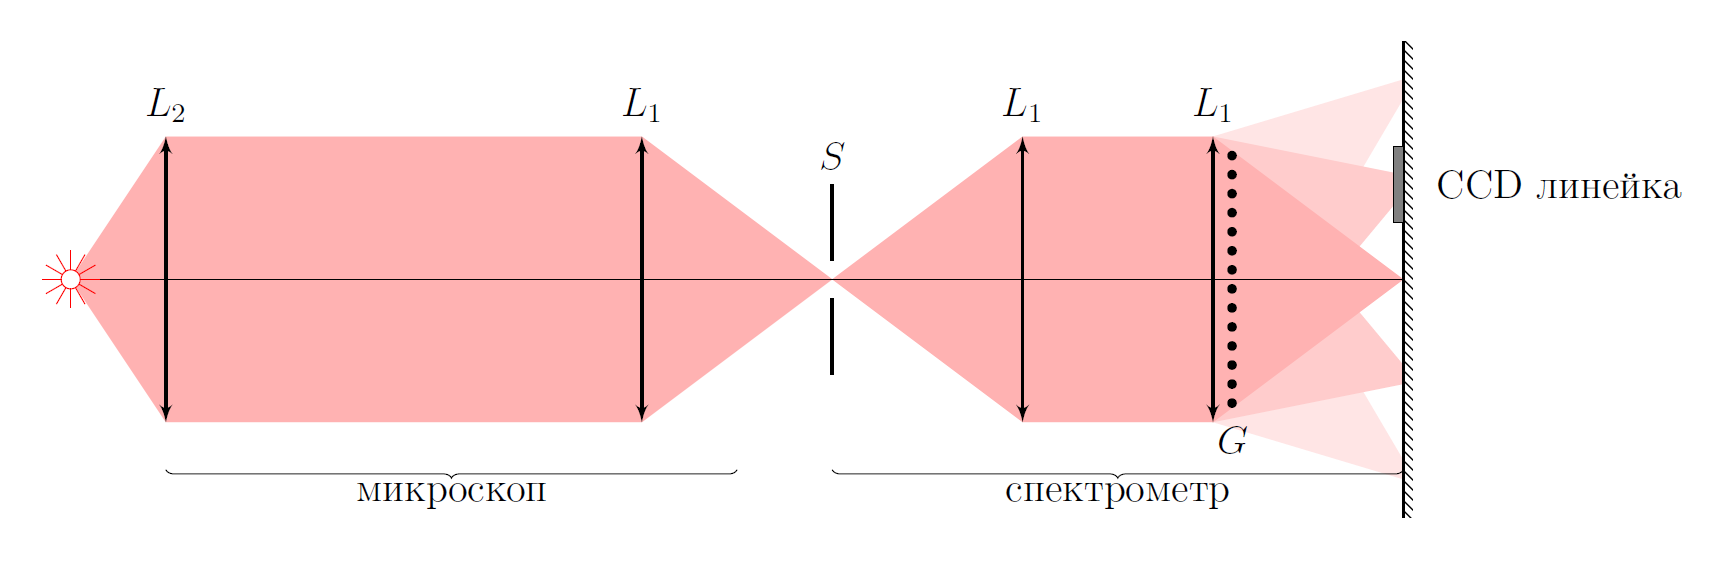
\includegraphics[width=0.72\textwidth]{E3_EN_assets/fig18.jpg}
    \caption{Modified optical design for fluorescence.}
\end{figure}

\problembox{C2}{Recalibrate the positions using the RGB-LED and save the spectra (R.csv, G.csv, B.csv) in folder C2.}{0.30}

\problembox{C3}{Express the average time $\tau$ between photon hits in terms of $\sigma, I_0,$ and $\omega_0$.}{0.20}

\problembox{C4}{Estimate the focus intensity $I_0$ and the time $\tau$ for the blue laser ($P_0=5$ mW, $d_0=2$ mm).}{0.90}

\problembox{C5}{Express the fluorescent power $P$ per unit volume in terms of $\sigma, I_0, \tau, \tau_0$ and $c$.}{0.40}

\problembox{C6}{Obtain the RhB fluorescence spectrum (100 $\mu$M) under blue laser excitation. Save as 405.csv and find $\lambda_{405,\max}$.}{0.50}

\problembox{C7}{Study $I_{405}(\lambda_{405,\max})$ as a function of the volume $V$ of solution added. Save as 405-$V$.csv.}{2.30}

\problembox{C8}{Plot the linearized graph and determine the absorption cross-section $\sigma_{405}$.}{1.50}

\problembox{C9}{Measure fluorescence spectra for four other concentrations $c$. Save as 405-$c$.csv.}{2.00}

\problembox{C10}{Plot $I_{405}(\lambda_{405,\max})$ versus $c$.}{1.20}

\problembox{C11}{Obtain and save (532.csv) the fluorescence spectrum under green laser excitation.}{0.20}

\problembox{C12}{On one graph, plot normalized absorption $A(E)$ and fluorescence $F(E)$.}{0.80}

\problembox{C13}{Draw the final qualitative Jablonski diagram for RhB.}{0.50}

\vspace{1em}
\noindent\textit{Source:} https://pho.rs/p/4541

\end{document}